% sample latex/latex2e file with lots of math, tables, figures, etc
% useful for writing papers
% genuine finger-typed files by Christina C. Christara

\documentclass[12pt]{article}
% \documentclass[12pt]{mypaper}

%\linespread{1.1} % for more than single spacing

% take more advantage of the size of paper
\addtolength{\topmargin}{-2cm}
\addtolength{\textheight}{4cm}
\addtolength{\evensidemargin}{-2cm}
\addtolength{\oddsidemargin}{-2cm}
\addtolength{\textwidth}{4cm}

% some standard packages
\usepackage{times}
\usepackage{graphics}
\usepackage{subfigure, epsfig}
\usepackage{rotate}
\usepackage{amssymb}
\usepackage{amsmath}
\usepackage{natbib} % bib
\usepackage{tikz} % neural networks
\usetikzlibrary{matrix,chains,positioning,decorations.pathreplacing,arrows}


\setlength{\parskip}{3mm}
% convenient abbreviations
\newcommand{\de}{\partial}

\begin{document}
\begin{center}
M.Sc. Research Project Proposal \\
% by \\
Bill (Mufan) Li \\
% M.Sc Candidate \\
Supervised by Professor Jeffrey Rosenthal \\
Department of Statistical Sciences \\
University of Toronto \\
Phone: (416)843-9179\\
Email: {\tt mufan.li@mail.utoronto.ca}\\
\bigskip\Large
{\bf Assessing GPA Measures From a Collaborative Filtering
Perspective}
\end{center}

Recent developments in machine learning have made significant 
contributions to a wide range of fields that are not 
traditionally considered data science.
Notably the Netflix competition have attracted a collective
effort in developing models that greatly improved prediction
of movie ratings by different users,
creating the best movie recommendation system at the time \cite{FeHeKh12}.
Similar to the Netflix rating data,
student grades in different courses follow the same structure,
allowing the application of the same machine learning techniques.
This research project aims to apply these
techniques to analyze the student grade dataset from \cite{BaRoYo14},
which contains complete transcripts of undergraduate students
from a major Canadian University.
Like predicting user ratings,
we are able to predict the grades for courses.
From the predictions, this project intends to analyze
the effect of choosing easier courses on student grades,
specifically by comparing the predicted grades of courses
students did not take against the courses taken 
within the same program.
By analyzing the variation in course difficulty,
these results could potentially improve curriculum design 
for educational institutions and admission procedure for
graduate programs.

Inference on missing data in the
student grade dataset falls directly under a collaborative
filtering (CF) problem, where a grade is only assigned for
some matches of students and courses.
The greatest difficulty of this type of problem is the sparsity
of data, where each student can only take a small subset of 
courses, leaving majority of potential course grades missing.
Additionally, data is not even distributed among courses, 
where some courses can have few attendance.
That being said, matrix factorization and restricted Boltzmann
machines techniques have been highly effective at collaborative filtering.
This project intends to investigate these two techniques and
the respective extensions with the student grade dataset.
This proposal will provide a brief overview of 
two main techniques that will be investigated,
as well as a discussion on several problems
this research project intend to address.

The most basic matrix factorization (MF) method,
known as singular value decomposition (SVD),
decomposes a large matrix into a product of two low-rank matrices.
Specifically for this problem, 
suppose there are $M$ students and $N$ courses,
then we define $\mathbf{A} \in \mathbb{R}^{M \times N}$ 
as the matrix of grades,
where $A_{ij}$ corresponds to the grade of 
student $i$ and course $j$.
We then seek two low-rank matrices 
$\mathbf{U} \in \mathbb{R}^{M \times d}$ 
and $\mathbf{V} \in \mathbb{R}^{N \times d}$ such that
%
\begin{equation}
	\mathbf{A} \approx \mathbf{UV}^\top .
\end{equation}

This is called a rank $d$ approximation of $\mathbf{A}$.
Note the value $A_{ij}$ is the dot product of
the $i$th row of $\mathbf{U}$ and 
the $j$th row of $\mathbf{V}$.
The row vectors may be interpreted as features,
i.e. row $i$ of $\mathbf{U}$ contains all the information
of student $i$.
% To optimize the rank $d$ approximation is 
% equivalent to minimizing the Frobenius norm of the difference
A common goal of optimization is to minimize the 
Frobenius norm of the difference for a rank $d$ approximation
$\left\Vert \mathbf{A - UV}^\top \right\Vert$,
defined by the square root of the
sum of squares of its entries \cite{FeHeKh12}.
In the case of collaborative filtering,
the Frobenius norm is not computed for missing entries.

% By the Eckart-Young Theorem, given a best rank $k-1$ approximation
% of $\mathbf{U}$ and $\mathbf{V}$, 
% a best rank $k$ approximation is obtained by adding
% a column to both $\mathbf{U}$ and $\mathbf{V}$
% such that the product minimizes 
% the Frobenius norm of the difference.

% This key result allows for iterative computation of 
% $\mathbf{U}$ and $\mathbf{V}$,
% reducing the complexity significantly.
% One approach, known as alternating least squares (ALS),
% fixes the column of interest of $\mathbf{U}$ 
% while using least squares
% to fit the column of $\mathbf{V}$, 
% then fixing $\mathbf{V}$ to fit $\mathbf{U}$,
% and alternates until convergence.
% The other approach calculates the gradient of
% the Frobenius norm
% with respect to all elements of $\mathbf{U}$ and $\mathbf{V}$,
% and perform steepest descent until convergence.
% While the optimization problem is non-convex,
% both approaches have been proven to reach satisfactory 
% local minima \cite{FeHeKh12}.

The greatest advantage of SVD is the simplicity of 
both implementation and inference,
where model optimization requires only least square
or gradient type methods,
and each missing value $A_{ij}$ is just 
the dot product of two row vectors of $\mathbf{U}$
and $\mathbf{V}$.
However, one significant weakness is SVD cannot incorporate 
student or course specific information besides the grades.
For example, a student's retaken or dropped courses cannot be easily
used by SVD.
Additionally, since the Frobenius norm cannot be computed for 
unknown values, SVD fails to optimize for regions where
the data is sparse.
One extension of MF is by defining a probabilistic distribution 
using the matrix product as the mean.
Under the probabilistic MF setup,
we can shift the mean of the distribution based on 
student and course specific information.
In fact, \cite{MnSa07} showed incorporating the probabilistic MF
successfully resolves both problems for the Netflix dataset.

On the other hand, restricted Boltzmann machines (RBM) is a
completely different approach to the problem.
A RBM is a Markov random field in the form of a bipartite graph,
where the joint probability follows a Boltzmann type distribution.
The bipartite graph structure creates two layers without
internal connections.
One layer, called the visible layer, contain the 
observed values of grades for a specific student.
These nodes are connected to the other layer, called the hidden layer,
with symmetrical weighted connections.
%
\def\layersep{2.5cm}
\begin{figure}[h]
\centering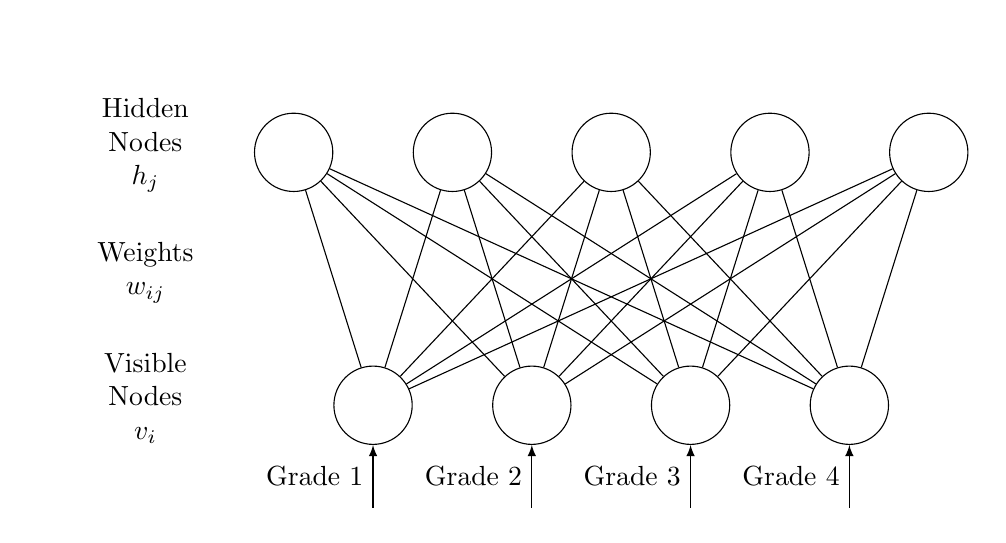
\begin{tikzpicture}[
plain/.style={
  draw=none,
  fill=none,
  },
net/.style={
  matrix of nodes,
  nodes={
    draw,
    circle,
    inner sep=10pt
    },
  nodes in empty cells,
  column sep=0pt,
  row sep=-1cm
  },
>=latex
]

\matrix[net] (mat)
{
|[plain]| \parbox{1.3cm}{\centering Hidden Nodes $h_j$} & & 
    |[plain]| & & |[plain]| & & |[plain]| & & |[plain]| & \\
|[plain]| \parbox{1.3cm}{\centering Weights $w_{ij}$}
    &|[plain]| &|[plain]| &|[plain]| &|[plain]| &
    |[plain]| &|[plain]| &|[plain]| &|[plain]| &|[plain]| \\
|[plain]| \parbox{1.3cm}{\centering Visible Nodes $v_i$} & 
    |[plain]| & & |[plain]| & & |[plain]| & & |[plain]| &\\
};
\foreach \ai [count=\mi ]in {3,5,7,9}
  \draw[<-] (mat-3-\ai) -- node[left] {Grade \mi} +(0cm,-1.3);
\foreach \ai in {2,4,...,10}
{\foreach \aii in {3,5,7,9}
  \draw[-] (mat-1-\ai) -- (mat-3-\aii);
}
\end{tikzpicture}

\caption{\label{fig:RBM}
A restricted Boltzmann machine (RBM) with 4 courses and 5 hidden
nodes for a specific student.
}
\end{figure}

Suppose the graph have $N$ visible nodes and $M$ hidden nodes,
with each visible node denoted $v_i$, hidden nodes denoted $h_j$, 
weights between two nodes $w_{ij}$,
$b_i$ and $a_j$ be bias parameters,
and $\sigma_i$ be the standard deviation of grades for each course.
Here each visible node $v_i$ represents the grade for course $i$,
where a specific student is fixed.
Let $\theta = \{ w_{ij},a_j,b_i,\sigma_i \} \; \forall i,j$,
$\mathbf{v} = \{v_i\} \; \forall i$,
and $\mathbf{h} = \{h_j\} \; \forall j$ denote the collections.
Additionally, we let the hidden nodes only take on binary values, 
i.e. $v_i \in \mathbb{R}, h_j \in \{0,1\}$.
We can then define the energy function and 
the joint distribution for the graph:
%
\begin{equation}
\begin{aligned}
    E(\mathbf{v},\mathbf{h}|\theta) &= 
        \displaystyle\sum_{i=1}^N \frac{(b_i - v_i)^2}{2 \sigma_i}
        - \displaystyle\sum_{i=1}^N \displaystyle\sum_{j=1}^M
             w_{ij} h_j \frac{v_i}{\sigma_i}
        - \displaystyle\sum_{i=j}^M a_j h_j \\
% \end{equation}
%
% The joint distribution for the graph is then defined
% by the Boltzmann distribution:
%
% \begin{equation}
    P(\mathbf{v},\mathbf{h}|\theta) &= 
        \frac{\exp\left[-E(\mathbf{v},\mathbf{h}|\theta)\right]}
        {\mathcal{Z}}
\end{aligned}
\end{equation}
%
where $\mathcal{Z}$ is the partition function normalizing
the distribution.
After marginalizing over the hidden nodes $\mathbf{h}$, 
we can find the gradient of the likelihood function
with respect to the parameters $\theta$
to perform steepest descent optimization.
Finding the gradient requires the use of Gibbs sampling,
although \cite{SaMnHi07} showed the approximate gradient
after very few iterations of Gibbs sampling is sufficient 
for optimization.
%
% \begin{equation}
%     \frac{\de P(\mathbf{v}|\theta)}{\de w_{ij}} = 
%         \mathbb{E}_{\text{data}} (v_i h_j) -
%         \mathbb{E}_{\text{model}} (v_i h_j)
% \end{equation}
%
% where $\mathbb{E}_{\text{data}}$ refers to expectation 
% of observing the case within data,
% and $\mathbb{E}_{\text{model}}$ is the expectation of 
% the current model with parameters $\theta$.
% Instead of using Gibbs sampling until convergence to find 
% $\mathbb{E}_{\text{model}}$, 
% \cite{SaMnHi07} uses $k$ iterations for a very good approximation
% of the gradient.
% This method is referred to contrastive divergence (CD) by the 
% authors in \cite{SaMnHi07}, where CD-$k$ refers to $k$ iterations
% used in Gibbs sampling.
% As a result, we have a very good algorithm optimize the
% RBM for likelihood.

To perform inference on a missing grade value,
one simply include an additional ``visible'' node $v_p$,
where the value is not known, 
but can be determined by the energy function:
%
\begin{equation}
% \begin{aligned}
    P(v_p|\mathbf{v}) \propto
        \displaystyle\sum_{\mathbf{h}} 
        \exp[-E(v_p,\mathbf{v},\mathbf{h})]
    % = \prod_{j=1}^M \left( 1 + 
    %     \exp\left[\sum_{i=1}^N w_{ij} v_i\right]
    %     \right)
% \end{aligned}
\end{equation}

Similar to probabilistic MF, RBM can also easily incorporate
student specific information within the model.
The RBM also has a natural extension into multiple layers
called deep belief networks (DBN) \cite{Sa09}.
This type of networks can represent much more complex 
relationships at a cost of more difficult optimization
and expensive computation for inferencing.

Both MF and RBM have been proven successful in 
the Netflix competition \cite{FeHeKh12}, 
therefore these techniques are expected to perform well 
in other collaborative filtering type problems.
In this project, we hope to address the following questions:
%
\begin{itemize} \itemsep0pt \parskip0pt
    \item Can the model correctly predict
        grades for future (or missing) courses given 
        previous year's (or incomplete) grades?
    \item Does the current GPA measure appropriately represent
        academic abilities when students select easier courses to 
        improve grades?
\end{itemize}

By leaving out some data during the optimization process,
predictions on these data can be tested.
This is commonly referred to the training data and test data
in machine learning.
With inference for missing grades, 
we can correctly assess the prediction power of the model,
answering the first question.
If grades are predicted for all courses that are available,
we can estimate a ``fair'' grade for students as if 
all students have taken the same courses.
This allows grading of student abilities on comparable grounds,
regardless of which courses the students have taken.
Finally, we can quantify the expected grade improvement 
due to the course selection by optimizing 
the choice of courses for all students in the dataset.
This results in a hypothetical grade,
comparing to the true grade answers the second question.
% Clearly student performance can be affected by much more
% complex and uncontrollable factors,
% but this hypothetical grade is sufficient for analysis of 
% whether easier courses systematically contribute unfairly to grades.

We intend to fully protect the privacy of students 
in the dataset during research 
by keep the data completely confidential,
only using it for agreed research purposes, 
and will not share it with anyone under any circumstances.
The project will use the data to provide valuable insights to 
educational institutions, 
potentially improving curriculum design and fair grading.

% This project provide valuable insights to educational 
% institutions by answering the two questions above.
% With these information, schools can improve course curriculum
% and fair grading.
% For admission and recruiting, this project provide
% a powerful tool to estimate a student's grade in courses.

% \medskip
% \noindent
% \small
% \setlength{\parskip}{0mm}
% {\bf References}

\bibliographystyle{plain}
\bibliography{proposal}


\end{document}






